\subsection{Proxy Re-Encryption}

\subsubsection{Introduction to Proxy Re-Encryption}

\begin{displayquote}{
  \textbf{"In a proxy re-encryption scheme a semi-trusted proxy converts a ciphertext for Alice into a ciphertext for Bob without seeing the underlying plaintext"}~\cite{greenateniese:2006:article}
}\end{displayquote}

Introduced as 'atomic proxy cryptography'~\cite{bbs:1998:book}, proxy re-encryption is the process of taking a message $M_a$, encrypted for a party $P_a$, and re-encrypting it such that it is readable by party $P_b$. Through the re-encryption process, the message is never decrypted by the proxy, such that the data is never revealed to any parties (including the proxy) other than the delegator and delegatees. This process relies on the functional relationship between the two ciphertexts, with the characteristics of the proxy re-encryption processed determined by the topology of this function.

\begin{figure}[H]
  \centering
  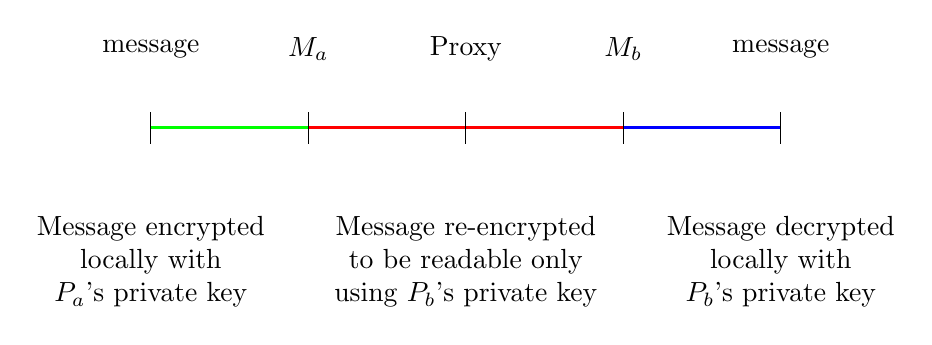
\begin{tikzpicture}

  \node at (0, 1)   {message} ;
  \node at (2, 1)   {$M_a$}   ;
  \node at (4, 1)   {Proxy}   ;
  \node at (6, 1)   {$M_b$}   ;
  \node at (8, 1)   {message} ;

  \draw [very thick, green] (0,0)   -- (2,0)   ;
  \draw [very thick, red]   (2,0)   -- (6,0)   ;
  \draw [very thick, blue]  (6,0)   -- (8,0)   ;
  \draw                     (0,-.2) -- (0, .2) ;
  \draw                     (2,-.2) -- (2, .2) ;
  \draw                     (4,-.2) -- (4, .2) ;
  \draw                     (6,-.2) -- (6, .2) ;
  \draw                     (8,-.2) -- (8, .2) ;

  \node[align=center, below] at (0, -1)%
    {Message encrypted\\locally with\\$P_a$'s private key};
  \node[align=center, below] at (4, -1)%
    {Message re-encrypted\\to be readable only\\using $P_b$'s private key};
  \node[align=center, below] at (8, -1)%
    {Message decrypted\\locally with\\$P_b$'s private key};

  \end{tikzpicture}
  \caption{
    Journey of a message using a proxy re-encryption scheme.
  }
\end{figure}


In figure \ref{fig:pre_example}, whether data is handled or manipulated by a fully trusted entity (a delegator or delegatee) or not is indicated using green/blue and red lines respectively.

The encrypted message $M_a$ is passed to the semi-trusted proxy along with the re-encryption key ( some $f(SK_a, PK_b)$\footnote{$SK_x$ represents the secret (private) key of a party $x$, $PK_x$ represents the public key of a party $x$.})

Below I discuss the contributions of various authors through the history of proxy re-encryption and the available schemes that might be suitable for a project focused on providing secure data sharing and storage.

% Delegation – allows a message recipient (keyholder) to generate a re-encryption key based on his secret key and the key of the delegated user. This re-encryption key is used by the proxy as input to the re-encryption function, which is executed by the proxy to translate ciphertexts to the delegated user's key. Asymmetric proxy re-encryption schemes come in bi-directional and uni-directional varieties.

% - In a bi-directional scheme, the re-encryption scheme is reversible—that is, the re-encryption key can be used to translate messages from Bob to Charlie, as well as from Charlie to Bob. This can have various security consequences, depending on the application. One notable characteristic of bi-directional schemes is that both the delegator and delegated party (e.g., Charlie and Bob) must combine their secret keys to produce the re-encryption key.
% - A uni-directional scheme is effectively one-way; messages can be re-encrypted from Bob to Charlie, but not the reverse. Uni-directional schemes can be constructed such that the delegated party need not reveal its secret key. For example, Bob could delegate to Charlie by combining his secret key with Charlie's public key.

% Transitivity – Transitive proxy re-encryption schemes allow for a ciphertext to be re-encrypted an unlimited number of times. For example, a ciphertext might be re-encrypted from Bob to Charlie, and then again from Charlie to David and so on. Non-transitive schemes allow for only one (or a limited number) of re-encryptions on a given ciphertext. Currently, there is no known uni-directional, transitive proxy re-encryption scheme. It is an open problem as to whether such constructions are possible.

\subsubsection{Atomic Proxy Cryptography}

Recognising that it is intuitive to expect any good cryptography scheme to disallow any untrusted party to re-encrypt a ciphertext, \cite{bbs:1998:book} suggests that perhaps it is desirable to allow re-encryption of a ciphertext, but only for specific delegatees. This is subject to doing so atomically, i.e. without revealing the underlying ciphertext, and without knowledge of the delegator or delegatee being exposed in the process. Conceptually this means that a delegator can encrypt once and have semi-trusted proxies re-encrypt for delegatees when desired.

Let's suppose we have a cryptography scheme whereby the following functions are observed:

\begin{itemize}
  \item $Gen(...)$: A generator of keys requiring arbitrary arguments
  \item $Encrypt(m, k)$: Allows the encryption of a message $m$ using the $k$ such that it is only decryptable by it's counterpart (or itself, if symmetric)
  \item $Decrypt(m, k)$: Allows the decryption of some encrypted message $m$ using the key $k$. Successful only if the message $m$ was encrypted (and intended for) the owner of the key $k$.
  \item $\Pi(m, rek_{a \rightarrow b})$: Allows the re-encryption of some encrypted message $m$ intended for the owner of key $a$ such that it is decryptable by the owner of key $b$.
  \item $ReGen(..., SK_a, PK_b)$: A generator of re-encryption keys requiring arbitrary arguments including keys required to decrypt
\end{itemize}}

As an example, imagine you wished to share an image privately between several friends. You encrypt this image and generate re-encryption keys for your friends (delegatees). Publishing the image and the keys means any third party (including the friends themselves) are able to re-encrypt the encrypted image such that a delegatee is able to decrypt it and view it.

The importance of the re-encryption function being atomic cannot be understated. The re-encryption function $\Pi$ alters the ciphertext effectively performing $\Pi(m_a, RK_{a \rightarrow b}) = Encrypt(Decrypt(m_a, SK_a), PK_b)$. However, if $\Pi$ were not atomic, the decryption of the message $m_a$ would reveal the plaintext content of the message to the proxy.

The following trust axioms apply to proxy re-encryption (assuming perfect implementation). The latter axiom only applies to symmetric key cryptography. Since the latter axiom is an undesirable property, we seek to only use asymmetric (public-key) cryptography to maintain security (of both parties).

\begin{itemize}
  \item A (unconditionally) trusts B since B can decrypt on behalf of A
  \item B trusts A since A can calculate $SK_b$ using the proxy key and $SK_a$. (\textit{Symmetric keys only})
\end{itemize}}

Given these properties, we will assume that asymmetric cryptography is a requirement of proxy re-encryption going forward.

\cite{bbs:1998:book} also discusses the notion of active versus passive proxy schemes distinguishing whether the delegatee has to cooperate or not in the creation of the proxy key. In practice, if the delegatee's public key is made available and is the only requirement from the delegatee then the delegator can delegate without the delegatee present, but otherwise, e.g. if the delegatee's secret key is required, the delegator needs the delegatee's cooperation to generate the proxy key required. Furthermore, in consideration of the delegator and delegatee's personally-identifying information, the proxy key can be distinguished as being transparent, translucent, or opaque depending on the ability of a third party to distinguish the two public keys the proxy is re-encrypting between.

\cite{bbs:1998:book} uses El Gamal encryption~\cite{elgamal:1985:article} as the basis for the proxy cryptography scheme suggested. A brief description of the protocol follows.

\paragraph{El Gamal Cryptography}

The El Gamal scheme includes the following functions:

\begin{itemize}
  \item $Gen(..., g, Z_n^*)$: A generator of keys requiring arbitrary arguments including some $g$, a generator in $Z_n^*$, itself a finite cyclic group of order $n$. Produces some secret key $\alpha$, whereby $0 \le \alpha \le n$, and a public key $g^\alpha$.
  \item $Encrypt(m, pk)$: Takes a random number, $r \in {0..n}$. Encrypts a message $m$ using the shared secret represented by $g^a^r = k$, A's public key to some random power. Outputs the tuple $(g^r, mk \text{ mod } n)$.
  \item $Decrypt(<pk, c>, sk)$: Decrypts some encrypted message $c$ using the secret key $sk$. Successful only if the message $c$ was encrypted for the owner of the key $sk$.
\end{itemize}

It is based on the Diffie-Helman protocol and relies on the discrete logarithm problem of $A = g^a$ being difficult.

\paragraph{BBS Scheme}

Similar to the standard El Gamal scheme, the Blaze, Bleumer, Strauss (BBS) scheme uses the same parameters but uses them to different effect.

As part of key generation, we now take $n$ to be of the form $2q + 1$ with $n$ itself prime. The generator is taken as above, with the secret key $a$ in ${0..n - 1}$, i.e. relatively prime to $n$. The inverse is also required for this scheme, so $a^{-1} \text{ mod } 2q$ is also calculated. The public key (published) is calculated as $g^a \text{ mod } n$. Encryption and decryption differ slightly to the standard El Gamal scheme:

\begin{itemize}
  \item $Encrypt(m, pk)$: Takes a random number, $r \in Z_{2q}^*$. Encrypts a message $m$ using the shared secret represented by $g^r = k$, A's public key to some random power. Outputs the tuple $(pk^r \text{ mod } n, mg^r \text{ mod } n)$.
  \item $Decrypt(<pk, c>, sk_a)$: Decrypts some encrypted message $c$ using the secret key $sk_a$. Successful only if the message $c$ was encrypted for the owner of the key $sk_a$, A. Uses the inverse of the secret key to yield $(pk^r \text{ mod } n)^{a^{-1}} = g^r (\text{mod } n)$. Taking the inverse of this result, we have the decryption key for the ciphertext: $mg^r \text{ mod } n(g^r (\text{mod } n))^{-1} = m$
\end{itemize}

Noting that the actual message is encrypted with some random $r$, this acts as a symmetric key during the encryption / decryption process. When the public key of the recipient is raised by $r$, this yields a result which is only decryptable by the intended recipient. Therefore we need a (proxy) function which is able to achieve the following:

$$
\begin{align}
& f(pk_a^r \text{ mod } n, re_{a \rightarrow b}) & &=& pk_b^r \text{ mod } n \\
\implies & f((g^a)^r \text{ mod } n, re_{a \rightarrow b}) & &=& (g^b)^r \text{ mod } n \\
\implies & re_{a \rightarrow b} & &=& g^{-a} \times g^{b}
\end{align}
$$

Note that the re-encryption process is more efficient than first decrypting the data and then re-encrypting the data with another key, since only one, atomic, exponentiation is required.

Given the reencryption key shown above ($g^{-a} \times g^{b}$), bilateral trust is required. $A$ can learn $B$'s key and vice versa. This is not desirable for this project and so we must look for alternative schemes which do not have this issue.

\subsubsection{Proxy Cryptography Revisited}

\cite{ivandodis:2003:inproceedings} suggested improved schemes which aim to address shortcomings of the original BBS scheme in their paper \textit{Proxy Cryptography Revisited}.



\subsubsection{Improved Proxy Re-encryption Schemes with Applications to Secure Distributed Storage~\cite{afgh:2006:article}}

\subsubsection{Unidirectional Chosen-Ciphertext Secure Proxy Re-Encryption~\cite{lv11:2011:article}}
